\documentclass[a4paper,14pt]{article}
\usepackage[utf8]{inputenc}
\usepackage[russian]{babel} 
\usepackage{graphicx} 
\usepackage{amsmath}
\usepackage{amssymb}
\usepackage{siunitx}% Для погрешностей
\usepackage{float}
\usepackage[colorlinks=true, linkcolor=blue]{hyperref}
\usepackage{enumitem}
\usepackage{longtable}
%\documentclass[fleqn]{article}

\renewcommand{\floatpagefraction}{0.99}
\renewcommand{\topfraction}{0.99}      

% Подключаем пакет для управления колонтитулами
\usepackage{scrlayer-scrpage}
\pagestyle{scrheadings}

%\clearpagemainheadfoot % Очищаем стандартные колонтитулы
\cfoot{\thepage}
% Настраиваем верхний правый угол (Right Head)
\rofoot{
\includegraphics[width=2.5cm]{Mir_insignia.png}}
% Вместо \rohead можно использовать:
% \lehead (левый верхний), \rofoot (правый нижний), \lefoot (левый нижний)

\title{ ЛАБОРАТОРНАЯ РАБОТА №5.1.

ИЗМЕРЕНИЕ СКОРОСТИ ЗВУКА В ВОЗДУХЕ
МЕТОДОМ БЕГУЩЕЙ ВОЛНЫ}


\author{Батанин Артём Александрович}
\date{\today}


\begin{document}

\maketitle

\newpage
\tableofcontents    
\newpage            



\section{Цель работы}
Цель работы: измерение зависимости амплитуды звуковой волны от расстояния до источника, определение скорости звука в воздухе методом бегущей волны и скорости потока воздуха.

\section{Оборудование}
Оборудование: установка для измерения скорости звука методом бегущей волны; генератор сигналов типа GFG 8255А, осциллограф типа TDS 1012, вентилятор.

\section{Задание 1. Измерение зависимости амплитуды волны от расстояния до источника}

Резонансная частота пьезоэлемента: 39.8кГц.
Измеренные зависимости представлены в \autoref{tab:tab1} \autoref{tab:tab2}, ниже приведены графики (Рис. \ref{fig:gr1})


\begin{figure}[H]
\centering
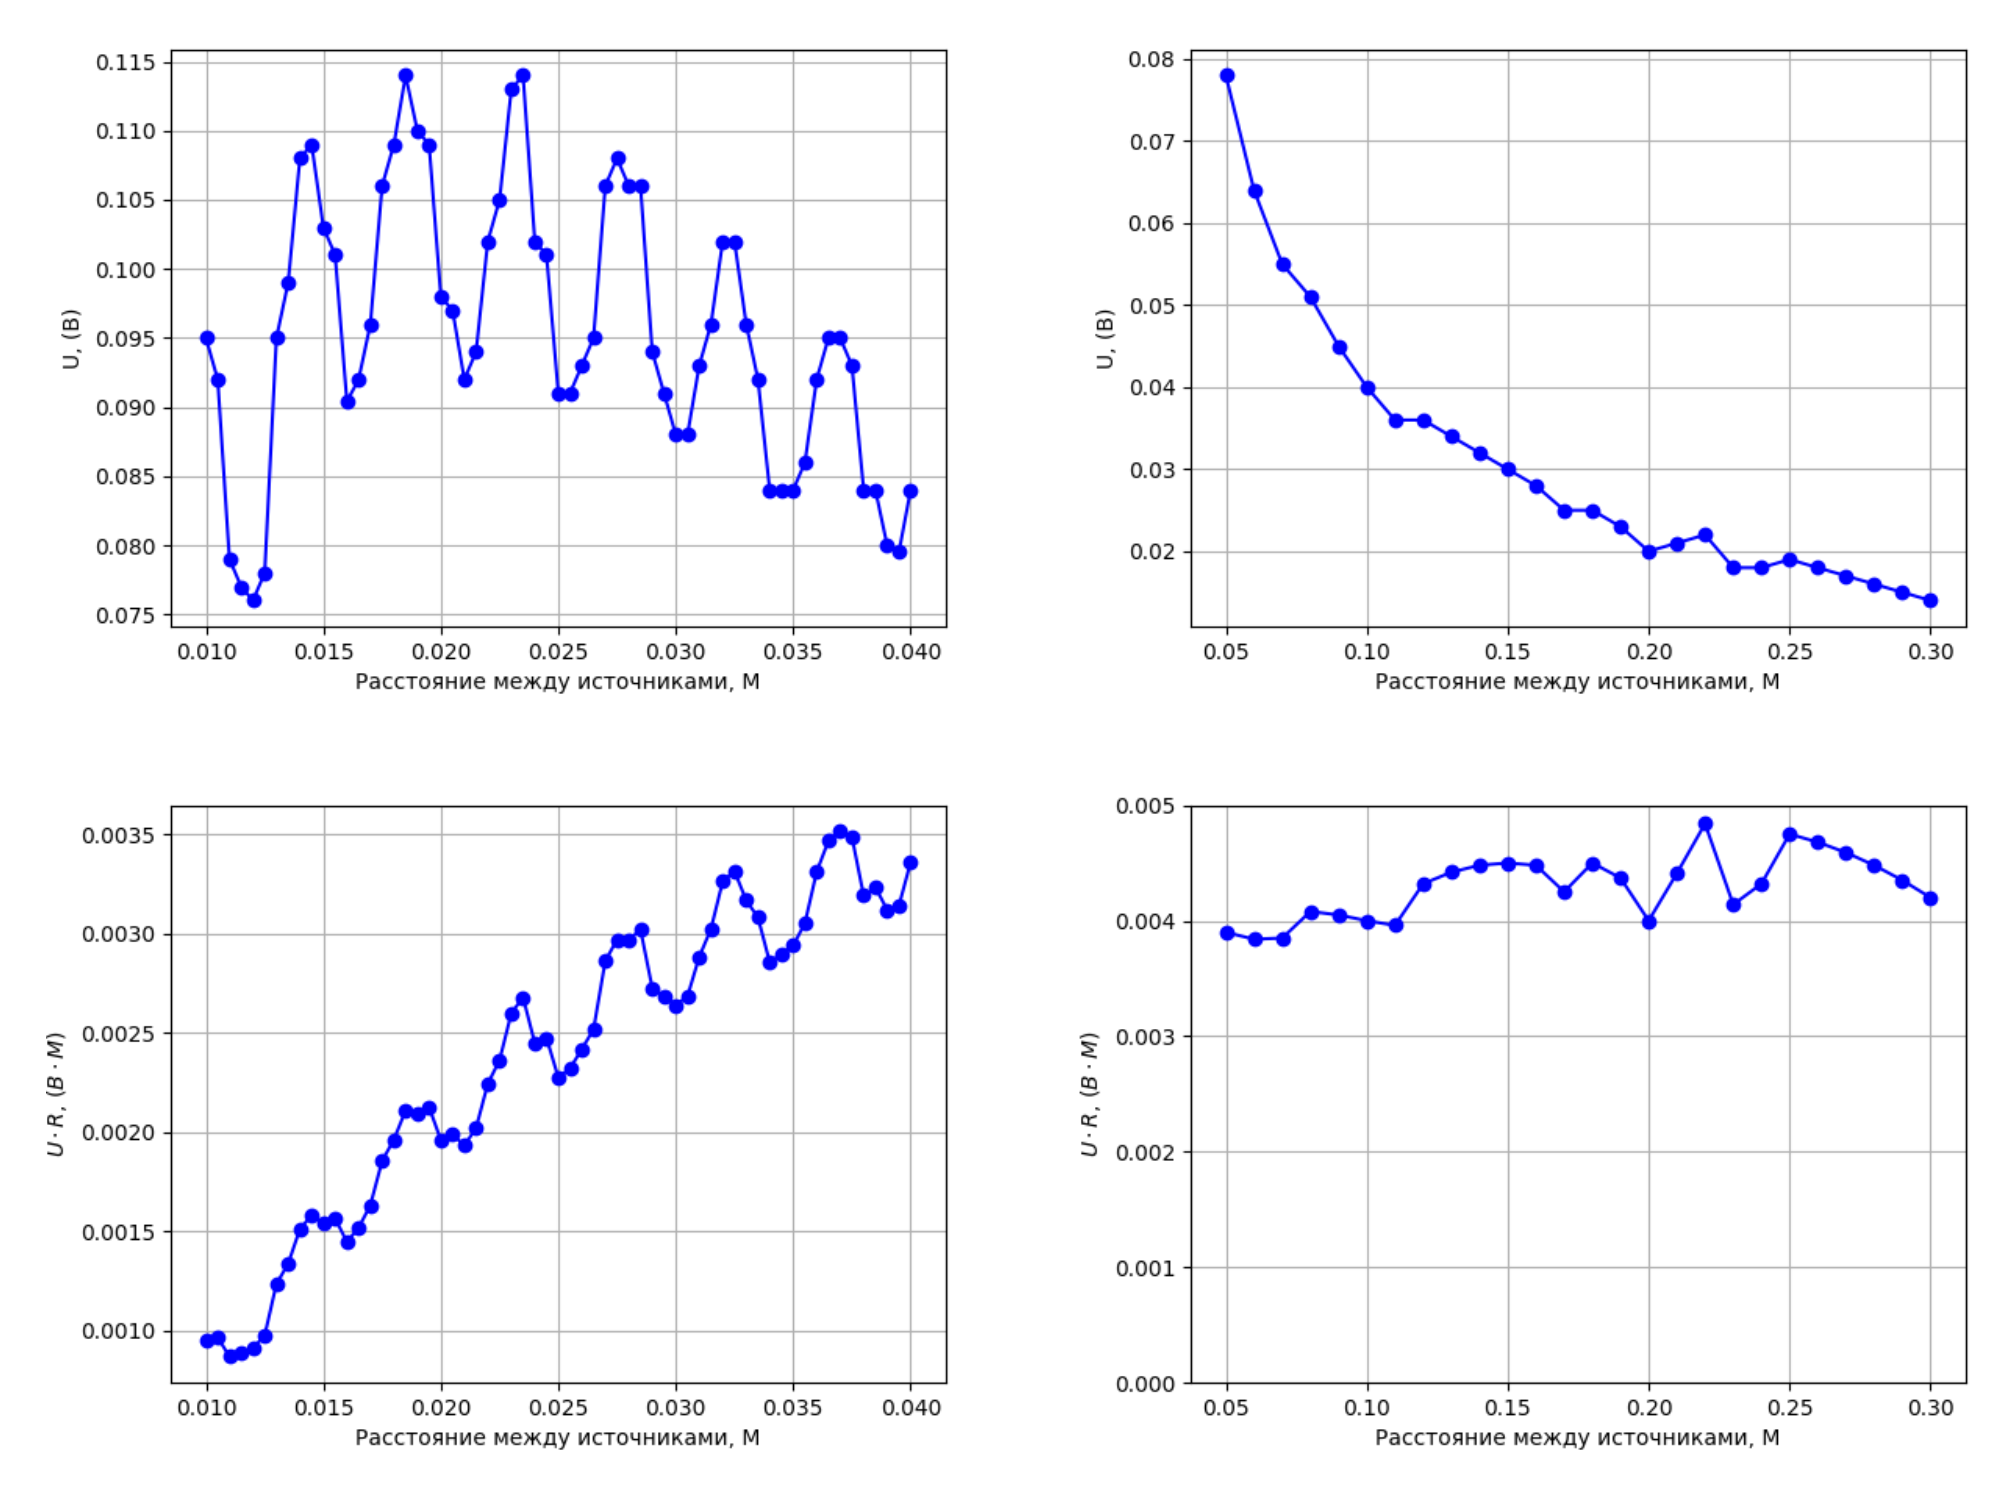
\includegraphics[width=1.2\linewidth]{grafix.png}
\caption{Зависимость амплитуды от расстоянии в ближней/дальней зоне}
\label{fig:gr1}
\end{figure}

%\begin{figure}[H]
%\centering
%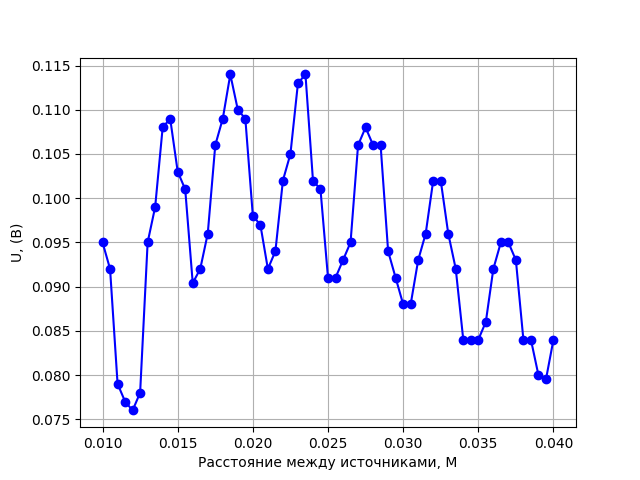
\includegraphics[width=0.49\linewidth]{bl.png}
%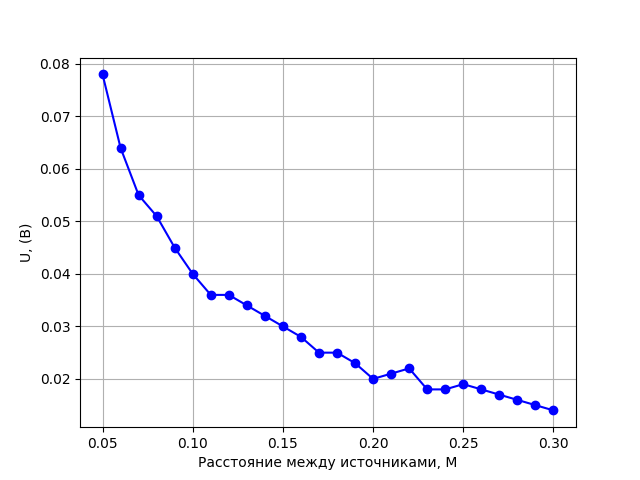
\includegraphics[width=0.49\linewidth]{d.png}
%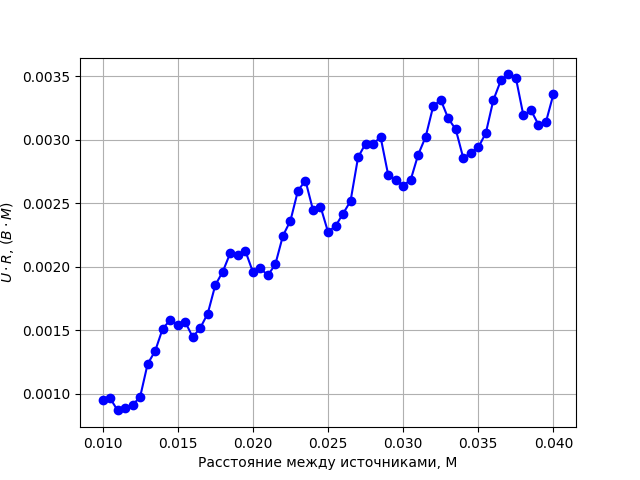
\includegraphics[width=0.49\linewidth]{blr.png}
%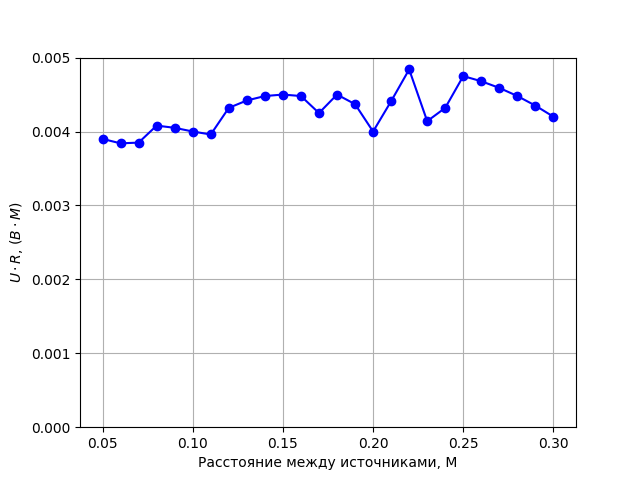
\includegraphics[width=0.49\linewidth]{dr.png}
%\caption{Зависимость амплитуды от расстоянии в ближней/дальней зоне}
%\label{fig:gr1}
%\end{figure}

Периодичность в ближней зоне объясняется интерференцией звука между излучателем и приёмником. Максимум достигается тогда, когда расстояние между излучателем и приёмником кратно длине волны звука, минимум, когда они сдвинуты на половину периода. Сигнал в ближней зоне не затухает как $\frac{1}{R^2}$ из-за того, что излучатель и приёмник - не точечные, а протяженные объекты, пренебрегать их размерами в ближней зоне нельзя.




















\section {Задание 2. Измерение скорости звука в воздухе}

Измеренные значения:

$r_1 = \num{107.75 \pm 0.025}$мм
$r_2 = \num{282.15 \pm 0.025}$мм

$f_1 = 39.80$кГц $\pm 0.9$Гц
$f_2 = 39.89$кГц $\pm 0.9$Гц


Оценка неопределённостей:
\begin{equation}
\begin{aligned}
\Delta C = 2\Delta r f/20 + \Delta f(r_2-r_1)/20
\label{error}
 \end{aligned}
\end{equation}

Оценка вклада неопределённости частоты и расстояния:
\begin{equation}
\begin{aligned}
\frac{\Delta C}{C} &= \frac{2\Delta r}{r_2 - r_1} + \frac{\Delta f}{f}\\
\frac{2\Delta r}{r_2 - r_1} &\approx 0.28\cdot 10^{-3}\\
\frac{\Delta f}{f} &\approx 0.02\cdot 10^{-3}\\
\label{error2}
 \end{aligned}
\end{equation}




Длина волны получилась $8.745 \pm $0.05 мм.
Измеренная скорость звука: $348.44 \pm $0.11 м/с.
Неопределенность измерений в действительности будет больше т.к. при расчетах выше не учитывался дрейф частоты (90 Гц).
С учётом дрейфа частоты неопределённость будет 0.9 м/с.

Скорость звука(табличная) 343 м/c.

Температура воздуха в помещении составляла 25°C. Согласно формуле
$C \approx 20.1 \sqrt{T}$ (T в кельвинах)
скорость звука приблизительно равна 346.9 м/с.



\section{Задание 3. Измерение скорости потока воздуха}
\subsection{Эксперимент}
Сдвиг фаз определялся методом фигур Лиссажу.
На изображении ниже \ref{fig:gr2} приведены измеренные сдвиги фаз, также они представлены в \autoref{tab:tab3}



\begin{figure}[H]
\centering
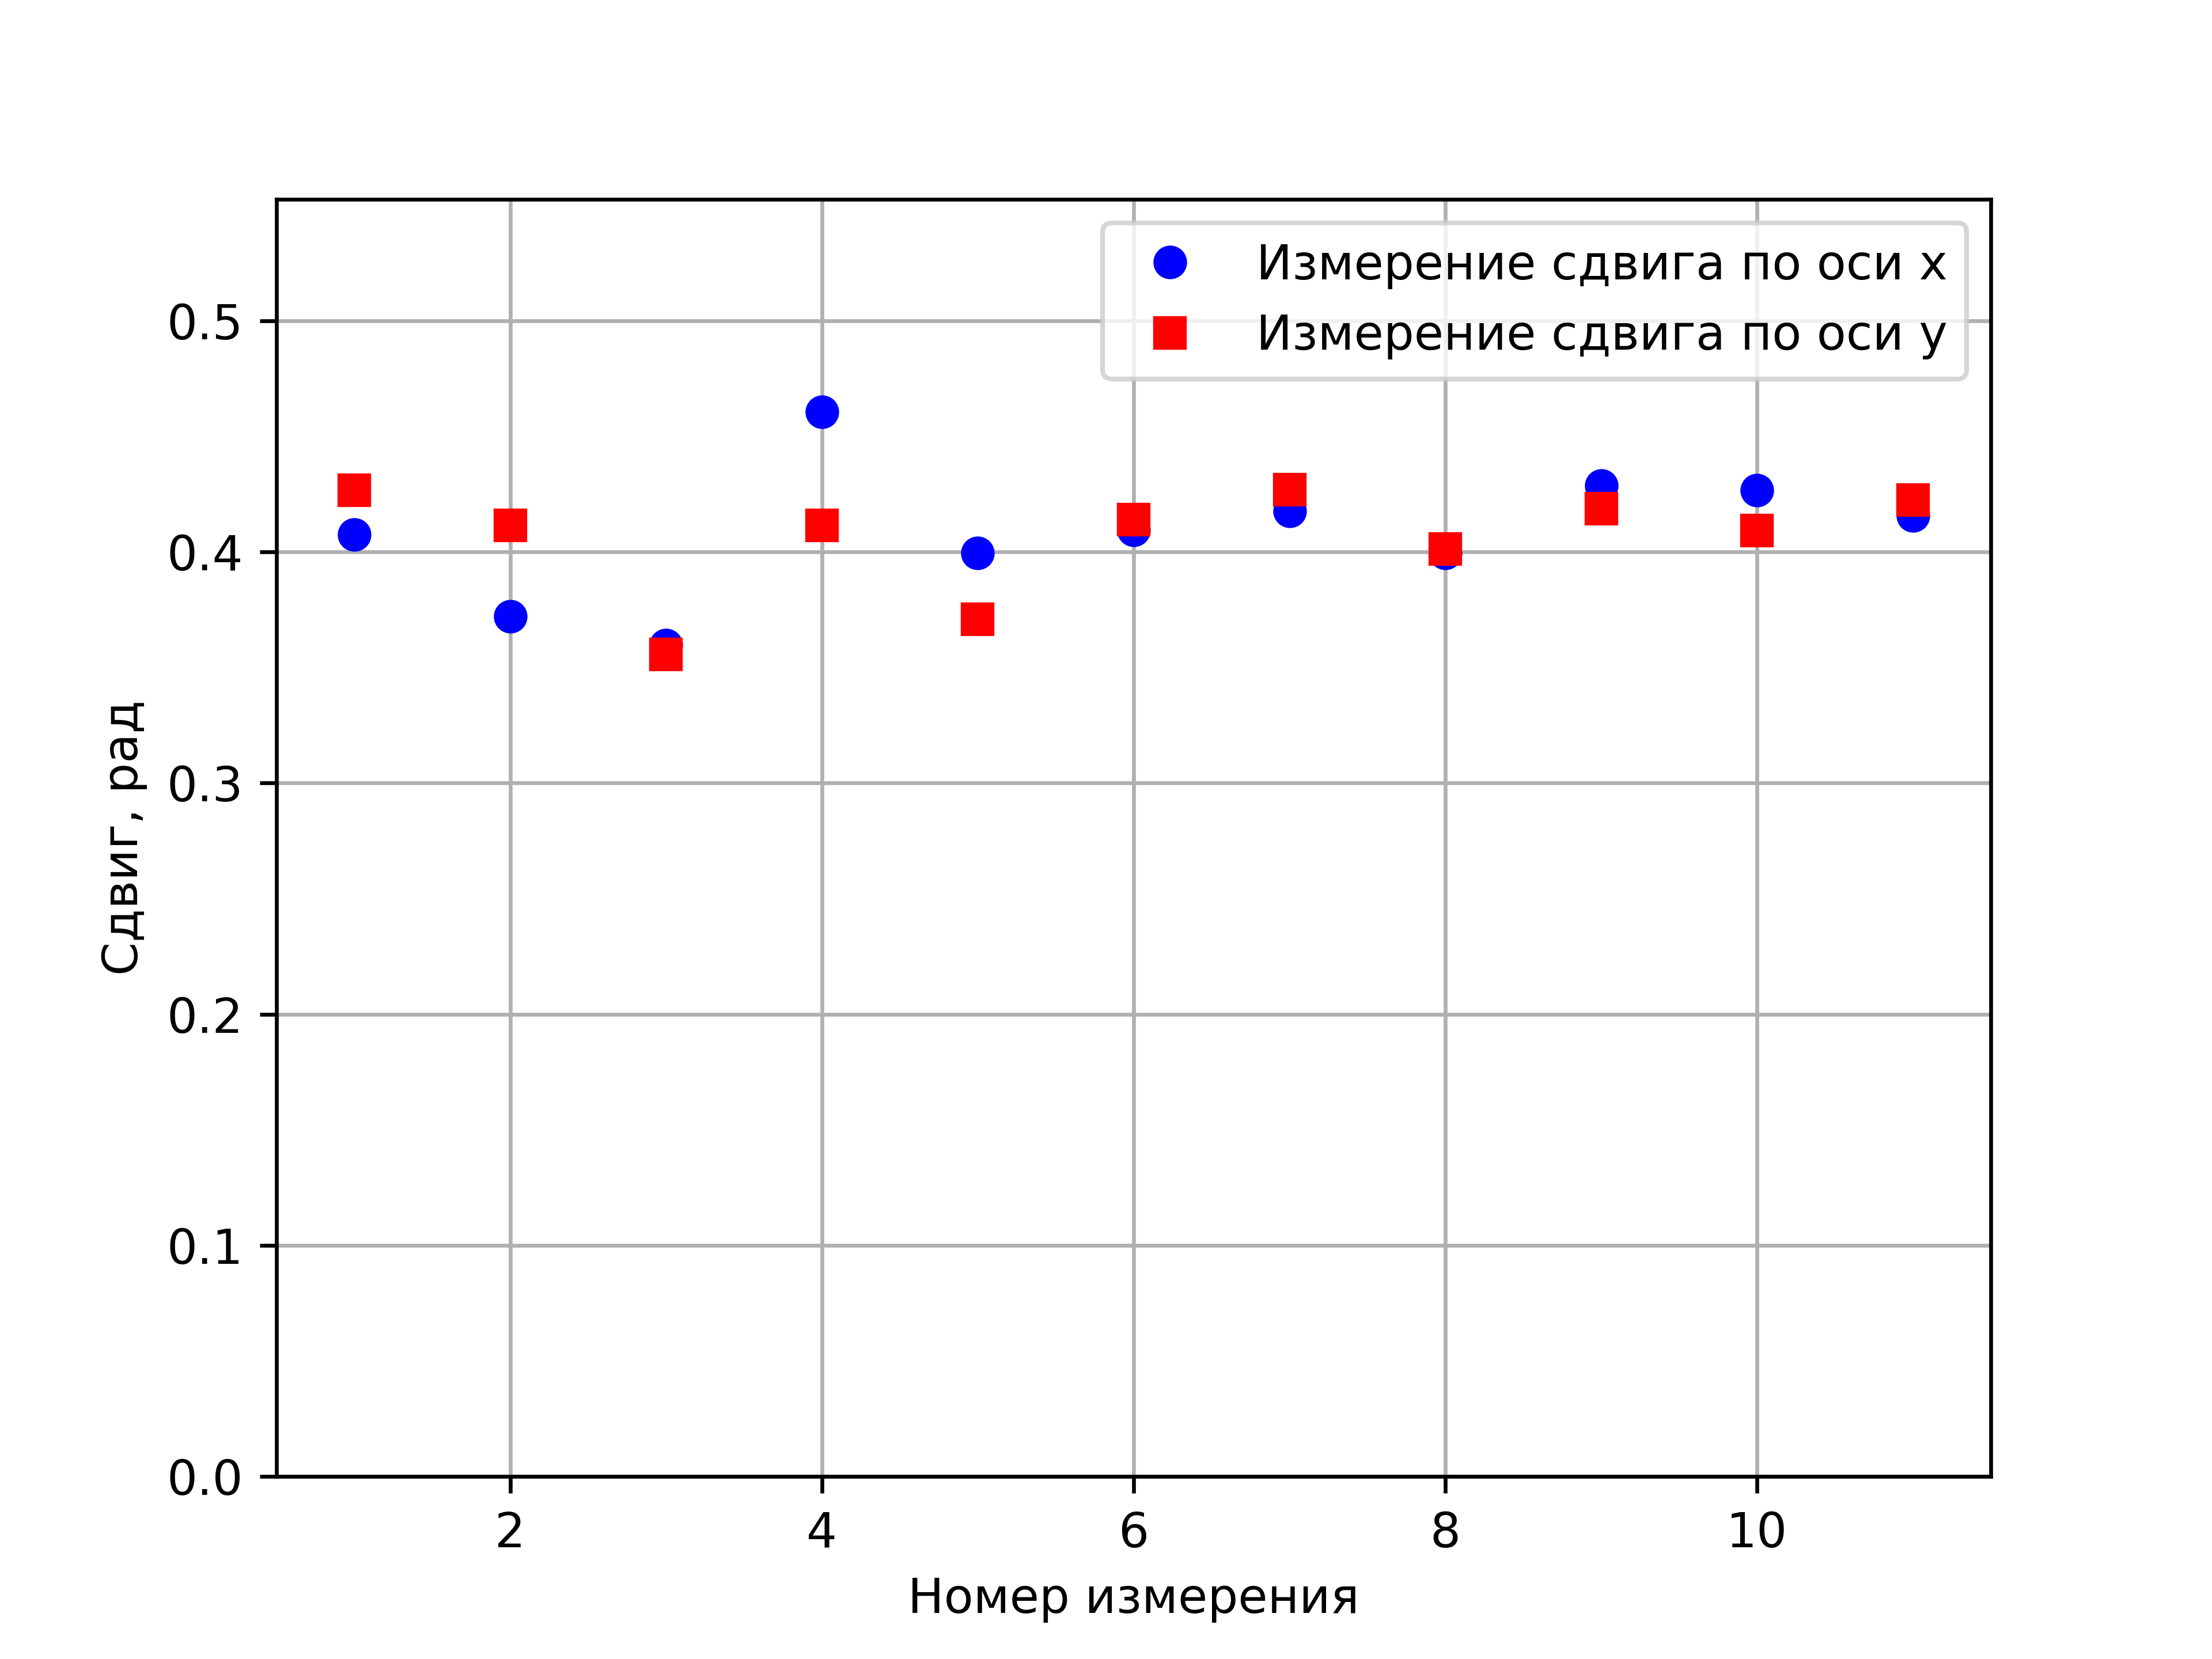
\includegraphics[width=1\linewidth]{phase_shift.png}
\caption{Сдвиг фаз}
\label{fig:gr2}
\end{figure}

\subsection{Анализ данных}
Ниже приведена оценка неопределенности измерения скорости ветра (в скобках указана неопределенность с учетом сдвига частоты генератора)
\begin{equation}
\begin{aligned}
\frac{\Delta V}{V} &= \frac{2\Delta C}{C} + \frac{\Delta f}{f} + \frac{\Delta r}{r} +  \frac{S_{\hat{\Delta \phi}}}{\Delta \phi} \\
\frac{\Delta C}{C} &\approx 0.32 \cdot 10^{-3} \text{ (или } 2.5 \cdot 10^{-3} \text{ )} \\
\frac{\Delta f}{f} &\approx 2.25 \cdot 10^{-5} \text{ (или }  2.5 \cdot 10^{-3} \text{ )}\\
\frac{\Delta r}{r} &\approx 0.17 \cdot 10^{-3}\\
\frac{S_{\hat{\Delta \phi}}}{\Delta \phi} &\approx 12.3 \cdot 10^{-3}\\
\label{error3}
 \end{aligned}
\end{equation}

Сдвиг фазы: $\Delta \phi = \num{0.408 \pm 0.005}$ рад.
Скорость звука получилась: $\num{1.364 \pm 0.019 \pm 0.028}$м/с (второй указана неопределенность с учетом дрейфа частоты)



\newpage
\section{Результаты измерений}


\begin{longtable}{|c|c|c|}
    % 1. Шапка на САМОЙ ПЕРВОЙ странице
    \caption{Зависимость амплитуды сигнала от расстояния до источника в ближней зоне} \label{tab:tab1} \\
    \hline
    \textbf{Расстояние до источника, мм} & Амплитуда, В & Произведение амплитуды и расстояния \\
    \hline
    \endfirsthead

    % 2. Шапка на ВСЕХ ПОСЛЕДУЮЩИХ страницах
    \hline
    \textbf{Расстояние до источника, мм} & Амплитуда, В & Произведение амплитуды и расстояния \\
    \hline
    \endhead

    % 3. Подвал на ПРОМЕЖУТОЧНЫХ страницах (указывает на продолжение)
    \hline
    \multicolumn{3}{|c|}{\textit{Продолжение на следующей странице...}} \\ \hline
    \endfoot

    % 4. Подвал на САМОЙ ПОСЛЕДНЕЙ странице таблицы
    \hline
    \endlastfoot

    % --- ТЕЛО ТАБЛИЦЫ (ваши данные) ---
10.0 & 0.095 & 0.95 \\ \hline
10.5 & 0.092 & 0.97 \\ \hline
11.0 & 0.079 & 0.87 \\ \hline
11.5 & 0.077 & 0.89 \\ \hline
12.0 & 0.076 & 0.91 \\ \hline
12.5 & 0.078 & 0.98 \\ \hline
13.0 & 0.095 & 1.23 \\ \hline
13.5 & 0.099 & 1.34 \\ \hline
14.0 & 0.108 & 1.51 \\ \hline
14.5 & 0.109 & 1.58 \\ \hline
15.0 & 0.103 & 1.54 \\ \hline
15.5 & 0.101 & 1.57 \\ \hline
16.0 & 0.0904 & 1.45 \\ \hline
16.5 & 0.092 & 1.52 \\ \hline
17.0 & 0.096 & 1.63 \\ \hline
17.5 & 0.106 & 1.86 \\ \hline
18.0 & 0.109 & 1.96 \\ \hline
18.5 & 0.114 & 2.11 \\ \hline
19.0 & 0.11 & 2.09 \\ \hline
19.5 & 0.109 & 2.13 \\ \hline
20.0 & 0.098 & 1.96 \\ \hline
20.5 & 0.097 & 1.99 \\ \hline
21.0 & 0.092 & 1.93 \\ \hline
21.5 & 0.094 & 2.02 \\ \hline
22.0 & 0.102 & 2.24 \\ \hline
22.5 & 0.105 & 2.36 \\ \hline
23.0 & 0.113 & 2.6 \\ \hline
23.5 & 0.114 & 2.68 \\ \hline
24.0 & 0.102 & 2.45 \\ \hline
24.5 & 0.101 & 2.47 \\ \hline
25.0 & 0.091 & 2.27 \\ \hline
25.5 & 0.091 & 2.32 \\ \hline
26.0 & 0.093 & 2.42 \\ \hline
26.5 & 0.095 & 2.52 \\ \hline
27.0 & 0.106 & 2.86 \\ \hline
27.5 & 0.108 & 2.97 \\ \hline
28.0 & 0.106 & 2.97 \\ \hline
28.5 & 0.106 & 3.02 \\ \hline
29.0 & 0.094 & 2.73 \\ \hline
29.5 & 0.091 & 2.68 \\ \hline
30.0 & 0.088 & 2.64 \\ \hline
30.5 & 0.088 & 2.68 \\ \hline
31.0 & 0.093 & 2.88 \\ \hline
31.5 & 0.096 & 3.02 \\ \hline
32.0 & 0.102 & 3.26 \\ \hline
32.5 & 0.102 & 3.31 \\ \hline
33.0 & 0.096 & 3.17 \\ \hline
33.5 & 0.092 & 3.08 \\ \hline
34.0 & 0.084 & 2.86 \\ \hline
34.5 & 0.084 & 2.9 \\ \hline
35.0 & 0.084 & 2.94 \\ \hline
35.5 & 0.086 & 3.05 \\ \hline
36.0 & 0.092 & 3.31 \\ \hline
36.5 & 0.095 & 3.47 \\ \hline
37.0 & 0.095 & 3.51 \\ \hline
37.5 & 0.093 & 3.49 \\ \hline
38.0 & 0.084 & 3.19 \\ \hline
38.5 & 0.084 & 3.23 \\ \hline
39.0 & 0.08 & 3.12 \\ \hline
39.5 & 0.0795 & 3.14 \\ \hline
40.0 & 0.084 & 3.36 \\ \hline

\end{longtable}

\begin{longtable}{|c|c|c|}

    \caption{Зависимость амплитуды сигнала от расстояния до источника в дальней зоне} \label{tab:tab2} \\
    \hline
    \textbf{Расстояние до источника, мм} & Амплитуда, В & Произведение амплитуды и расстояния \\
    \hline
    \endfirsthead


    \hline
    \textbf{Расстояние до источника, мм} & Амплитуда, В & Произведение амплитуды и расстояния \\
    \hline
    \endhead


    \hline
    \multicolumn{3}{|c|}{\textit{Продолжение на следующей странице...}} \\
    \hline
    \endfoot


    \hline
    \endlastfoot


50.0 & 0.078 & 3.9 \\ \hline
60.0 & 0.064 & 3.84 \\ \hline
70.0 & 0.055 & 3.85 \\ \hline
80.0 & 0.051 & 4.08 \\ \hline
90.0 & 0.045 & 4.05 \\ \hline
100.0 & 0.04 & 4.0 \\ \hline
110.0 & 0.036 & 3.96 \\ \hline
120.0 & 0.036 & 4.32 \\ \hline
130.0 & 0.034 & 4.42 \\ \hline
140.0 & 0.032 & 4.48 \\ \hline
150.0 & 0.03 & 4.5 \\ \hline
160.0 & 0.028 & 4.48 \\ \hline
170.0 & 0.025 & 4.25 \\ \hline
180.0 & 0.025 & 4.5 \\ \hline
190.0 & 0.023 & 4.37 \\ \hline
200.0 & 0.02 & 4.0 \\ \hline
210.0 & 0.021 & 4.41 \\ \hline
220.0 & 0.022 & 4.84 \\ \hline
230.0 & 0.018 & 4.14 \\ \hline
240.0 & 0.018 & 4.32 \\ \hline
250.0 & 0.019 & 4.75 \\ \hline
260.0 & 0.018 & 4.68 \\ \hline
270.0 & 0.017 & 4.59 \\ \hline
280.0 & 0.016 & 4.48 \\ \hline
290.0 & 0.015 & 4.35 \\ \hline
300.0 & 0.014 & 4.2 \\ \hline

\end{longtable}







\begin{longtable}{|c|c|c|c|c|c|c|}

    \caption{Измеренные значения сдвига фаз} \label{tab:tab3} \\
    \hline
    \textbf{Номер измерения} & $x_0$ (мВ) & $x_{max}$ (мВ) & $y_0$ (мВ) & $y_{max}$ (мВ) & $\Delta \phi_x$  (рад) & $\Delta \phi_y$ (рад)  \\
    \hline
    \endfirsthead


    \hline
    \textbf{Номер измерения} & $x_0$ (мВ) & $x_{max}$ (мВ) & $y_0$ (мВ) & $y_{max}$ (мВ) & $\Delta \phi_x$  (рад) & $\Delta \phi_y$ (рад)  \\
    \hline
    \endhead


    \hline
    \multicolumn{3}{|c|}{\textit{Продолжение на следующей странице...}} \\
    \hline
    \endfoot


    \hline
    \endlastfoot


1 & 4.2 & 10.6 & 6.0 & 14.5  & 0.407 & 0.427 \\ \hline
 2 & 4.0 & 11.0 & 5.84 & 14.6  & 0.372 & 0.412 \\ \hline
 3 & 3.8 & 10.8 & 5.92 & 17.0  & 0.36 & 0.356 \\ \hline
 4 & 4.8 & 10.8 & 6.8 & 17.0  & 0.461 & 0.412 \\ \hline
 5 & 4.2 & 10.8 & 6.16 & 17.0  & 0.399 & 0.371 \\ \hline
 6 & 4.3 & 10.8 & 6.84 & 17.0  & 0.409 & 0.414 \\ \hline
 7 & 4.3 & 10.6 & 7.04 & 17.0  & 0.418 & 0.427 \\ \hline
 8 & 4.2 & 10.8 & 6.64 & 17.0  & 0.399 & 0.401 \\ \hline
 9 & 4.24 & 10.2 & 7.4 & 18.2  & 0.429 & 0.419 \\ \hline
 10 & 4.18 & 10.1 & 7.4 & 18.6  & 0.427 & 0.409 \\ \hline
 11 & 4.08 & 10.1 & 4.1 & 10.0  & 0.416 & 0.422 \\ \hline

\end{longtable}





\end{document}